In this section several parameter variables are used. Each variable has a subscript indicating which particles were used in its calculations and a superscript indicating the galaxy radius. For simplicity, the values calculated using a radius of 15 \% of the virial radius are marked with superscript 1. Values calculated using all the particles bound to the subhalo as identified by SUBFIND and which are available in the data catalog on the TNG webpage have the superscript SF.

\subsection{Stellar-to-halo-mass relation}

To study the effect of the choice in stellar mass definitions, several possible galaxy radii have been used to calculate the galaxy's total stellar mass. The largest possible value is that of SUBFIND, where the mass is the sum of all the stellar particles bound to the subhalo ($M^{SF}_\ast$). The other definitions of stellar mass which were studied are compared to this value. These definitions are the stellar mass within 15 \% of the virial radius ($M_\ast^1$), the stellar mass within 30$\,$ kpc ($M_\ast^{30kpc}$) and the stellar mass within twice the SUBFIND half mass radius ($M_\ast^{2Rhm}$)\footnote{These values are available in the TNG group catalog}. These are all definitions which are commonly used in works where TNG data is employed. The results for the fractional difference in stellar mass measurements are presented in Figure \ref{SM_fSM}.

The most obvious result is the significant difference between $M^{SF}$ and $M_\ast^{2Rhm}$, with the latter being at least 20 \% smaller for all stellar masses. $M_\ast^1$ give the highest values of stellar mass of the three mass definitions, and is essentially indistinguishable from the SUBFIND values at masses below $10^{10.5} M_{\odot}$. The stellar mass within 30$\,$ kpc is similar to $M^1_\ast$ for galaxies with total stellar masses $M^{SF}_\ast < 10^{10.7} M_{\odot}$. For more massive galaxies there is an increasingly large difference between the two as well as compared to SUBFIND. At the higher mass end ($M^{SF}_\ast > 10^{11} M_{\odot}$), $M^1_\ast$ is about 10-15 \% smaller than SUBFIND, $M_\ast^{30kpc}$ is 12-40 \% smaller while $M_\ast^{2Rhm}$ is approximately 30 \% smaller. 


A direct comparison of stellar masses found in galaxies between TNG and some other study would therefore be significantly affected by the choice of how stellar mass is defined. This is one of the reasons why galaxy properties are not directly comparable and we have to look at the trends in the properties rather than the exact values. However, this might also affect property relations, depending on how other properties are calculated. It is therefore interesting to see if other galaxy properties have a similar dependency on galaxy size definitions.

\begin{figure}
    \centering
    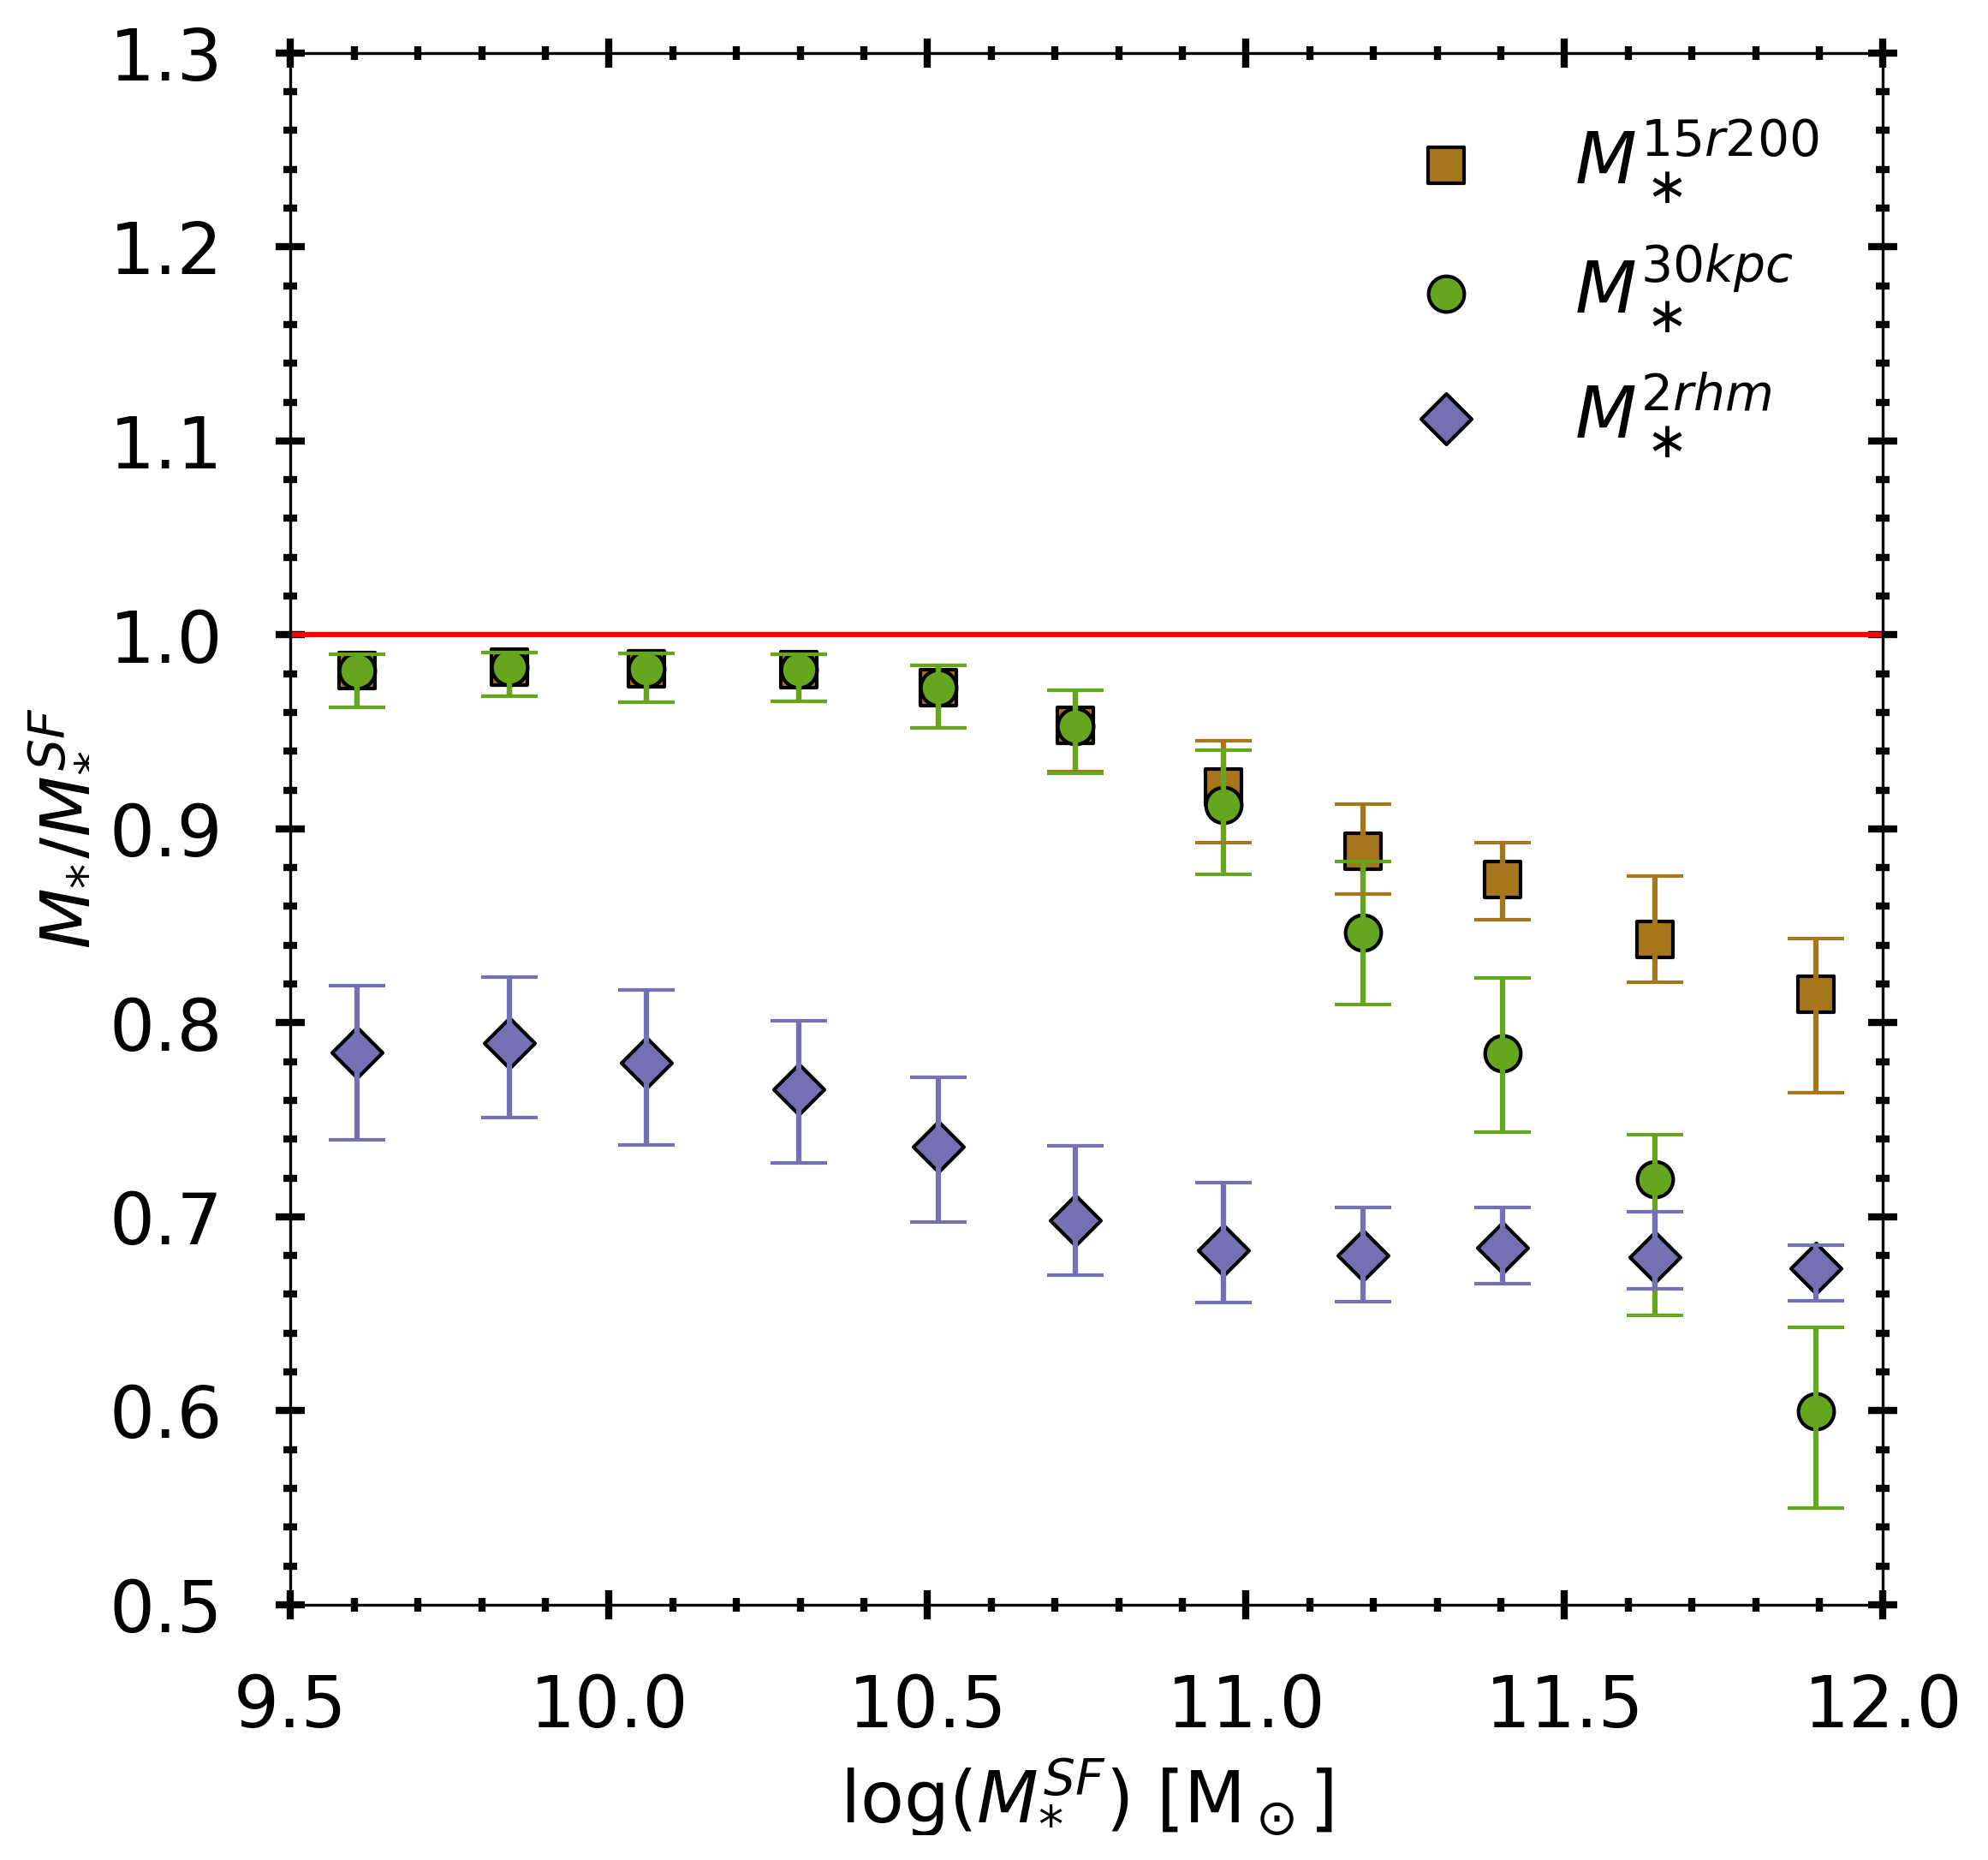
\includegraphics[width=0.9\textwidth]{images/SM_fSM.png}
    \caption{The fractional difference between the stellar mass of the galaxy using different definitions of galaxy size and the total mass of all stellar particles bound to the subhalo as identified by SUBFIND. Median values with 25-75 percentile error bars are given for the stellar mass within 15 \% of the virial radius ($M_\ast^1$, purple squares), the stellar mass within 30$\,$ kpc ($M_\ast^{30kpc}$, green circles) and the stellar mass within twice the SUBFIND half mass radius ($M_\ast^{2Rhm}$, orange diamonds)}
    \label{SM_fSM}
\end{figure}


In Figure \ref{shmr} the SHM relation is shown for two different definitions of stellar mass in TNG ($M^{SF}_\ast$ and $M^{30kpc}$) along with the best fits from \textcite{Behroozi2013} and \textcite{Zanisi2019}. By using the smaller galaxy size when calculating the stellar mass for TNG galaxies, the results are more similar to the most recent observations. This showcases the importance of making it clear which stellar mass definition was chosen. However, all the different definitions explored here do overestimate the stellar mass compared to observations when looking at the very largest galaxies. Comparing with the newer observational data makes the difference much smaller, and within the error estimates, but it should still be considered whether the feedback mechanisms implemented in TNG tend to give the largest galaxies too much stellar mass. 

\begin{figure}
    \centering
    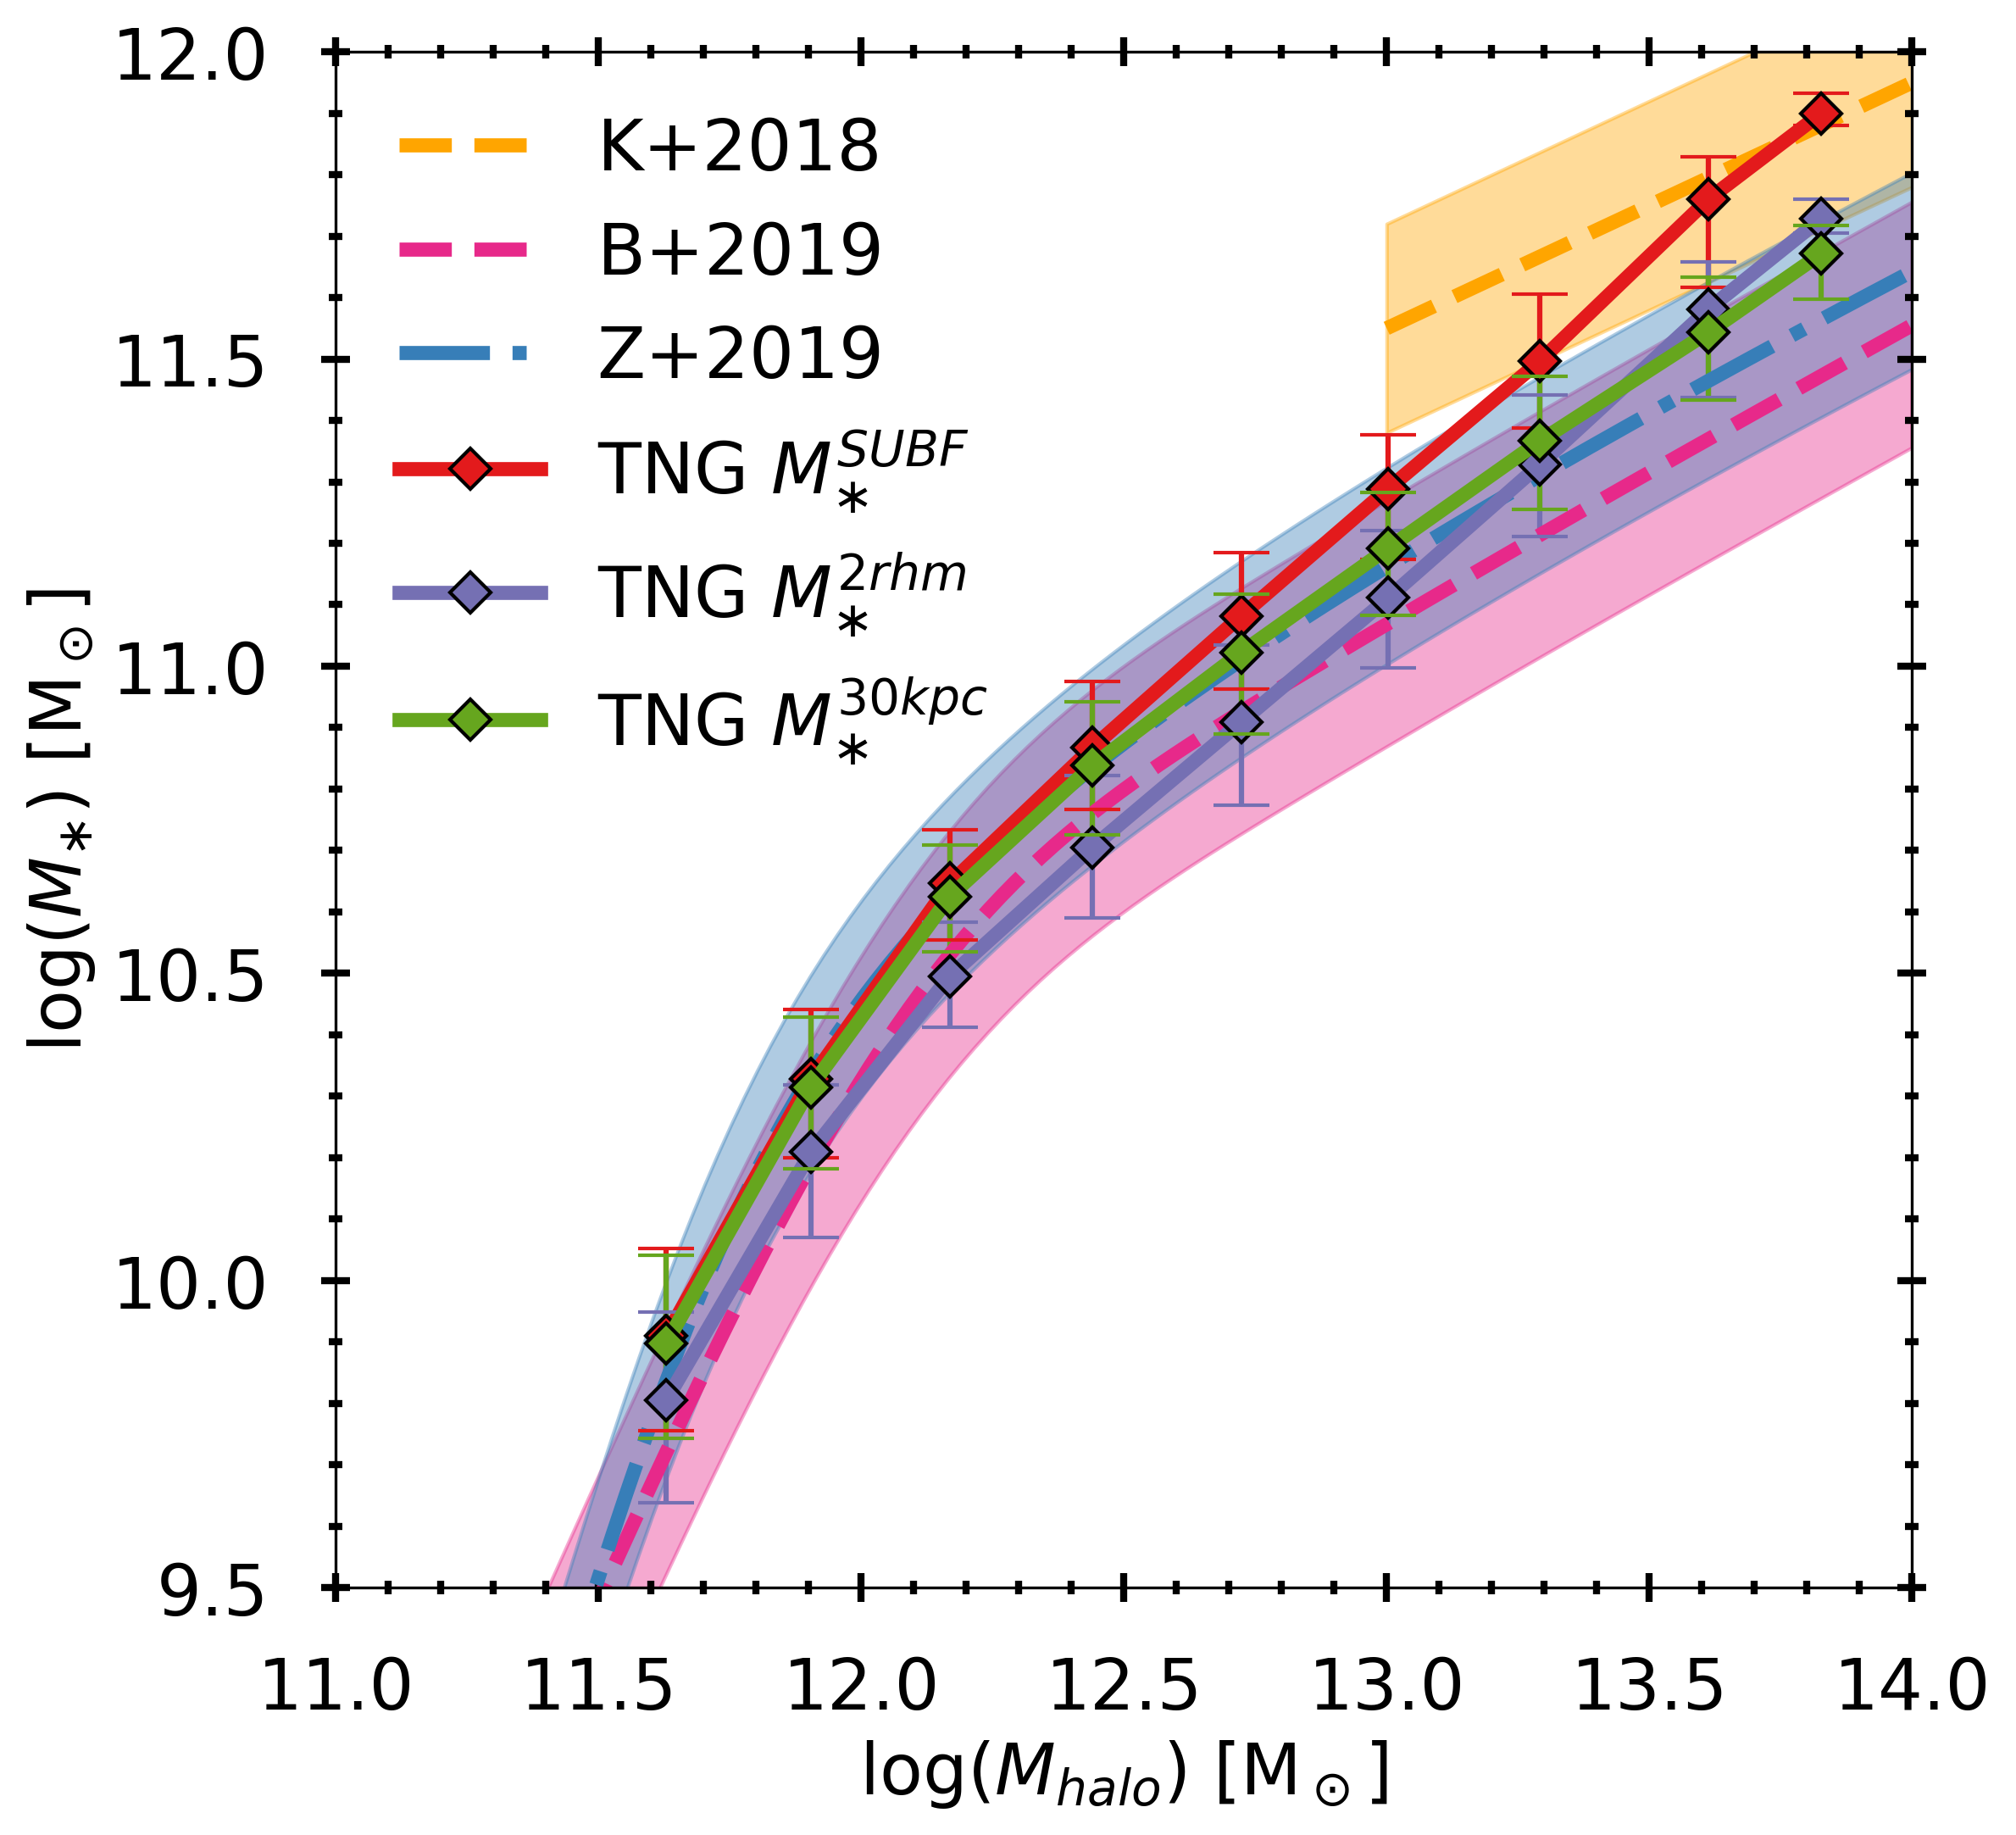
\includegraphics[width=0.9\textwidth]{images/shmr.png}
    \caption{The SHM relation of TNG is shown (orange dots), along with median points (blue line and markers) with error bars showing the 25-75 percentile. The best fit from abundance matching from \textcite{Behroozi2013} (red dashed line) and \textcite{Zanisi2019} (green dashed line) are also shown.}
    \label{shmr}
\end{figure}

\subsection{Mass-size-velocity relations}

\subsubsection{Size}
The half-mass radius will of course be affected by the definition of stellar mass, as it is defined as the radius within which half the stellar mass of the galaxy is found. This can be seen in Figure \ref{SM_R_TNG} in which the stellar half-mass radius and the projected half-mass radius is plotted for different galaxy size definitions. There is a large scatter in this function, and the resulting trends lie within the 25-75 percentile of each other. However, it is still clear that there is a difference in the slope of the relation for the $M_\ast > 10^{11} M_{\odot}$ regime. It is also interesting to compare the two methods of calculating projected 2D half-mass radii. The only possible method using the SUBFIND catalog is to use the approximate relation $R_{\ast, 2D} \approx 3/4 \times r_{\ast, 3D}$. When using the particles, one can project the galaxies in three orthogonal directions and calculate the average 2D half-mass radius. The results show that multiplying by a factor of $3/4$ is an excellent approximation to the projected stellar half-mass radius.

In Figure \ref{SM_R}, the TNG projected half mass radii are compared against the data from the SAMI survey. The TNG simulation produces galaxies with half-mass radii that are slightly larger than the SAMI effective radii at lower stellar masses. At high stellar masses the SUBFIND values are higher than those of the fixed aperture of 30 kpc, and the latter is a better fit for the observational data. There is however a large scatter in both observation and simulation results as well as uncertainities which are not accounted for in this study. Keeping this in mind, the similarity in the stellar mass - effective radius relation between observation and TNG is remarkable. 

The stellar mass-size relation for early and late type galaxies is shown in Figure \ref{SM_R_morph}. The half-mass radii for late type galaxies are larger than for early types with similar mass, as expected. An interesting feature is that for both late and early types, the TNG galaxies have smaller half-mass radii compared to the SAMI effective radii in the stellar mass range $10^{10.2} M_{_\odot} - 10^{10.7} M_{_\odot}$, while this effect is not really seen in the plot with all the galaxies included. This must be attributed to the intermediate-type galaxies, which comprise about half the TNG galaxy sample and are then pushing the mean of the half-mass radii upwards in that regime. 

\begin{figure}
    \centering
    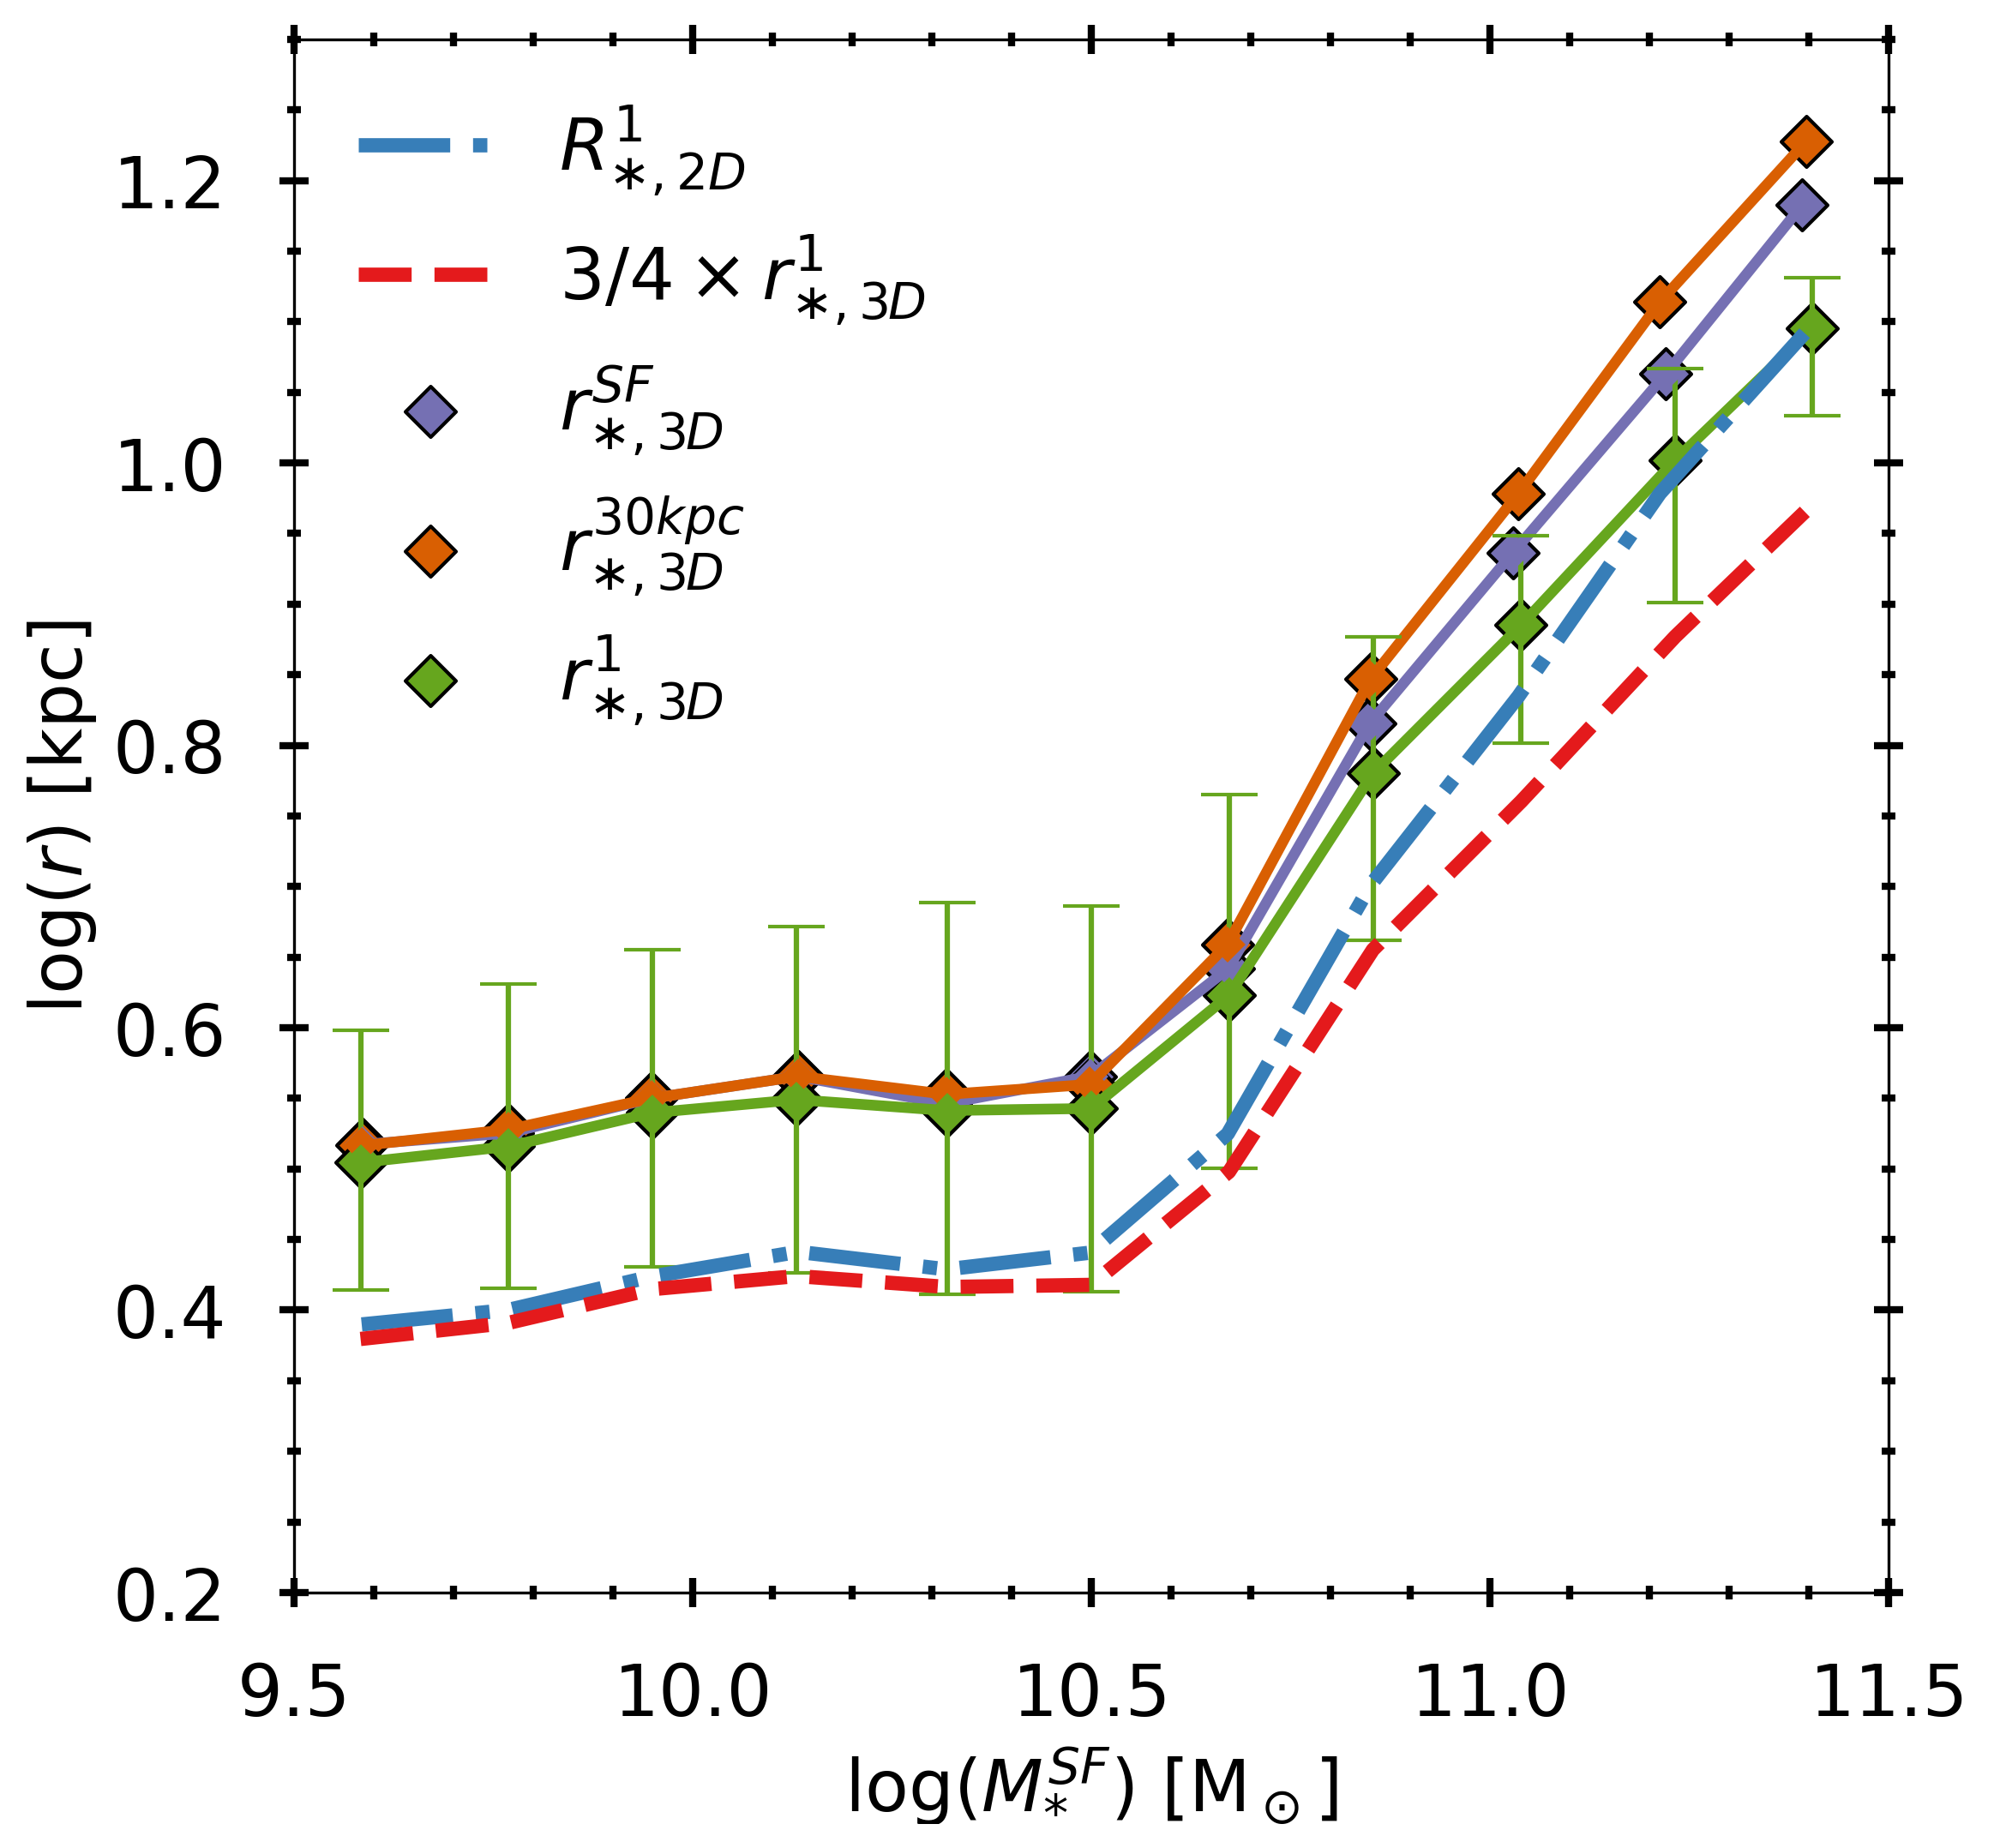
\includegraphics[width=0.9\textwidth]{images/SM_R_tng.png}
    \caption{The size-mass relation for different galaxy size definitions in TNG. Solid lines with dots show the 3D radius and dashed lines are 2D projected radius. The 25-75 percentile error bars are shown for $r^{1}_{*, 3D}$ only, as it is similar in all definitions.}
    \label{SM_R_TNG}
\end{figure}


\begin{figure}
    \centering
    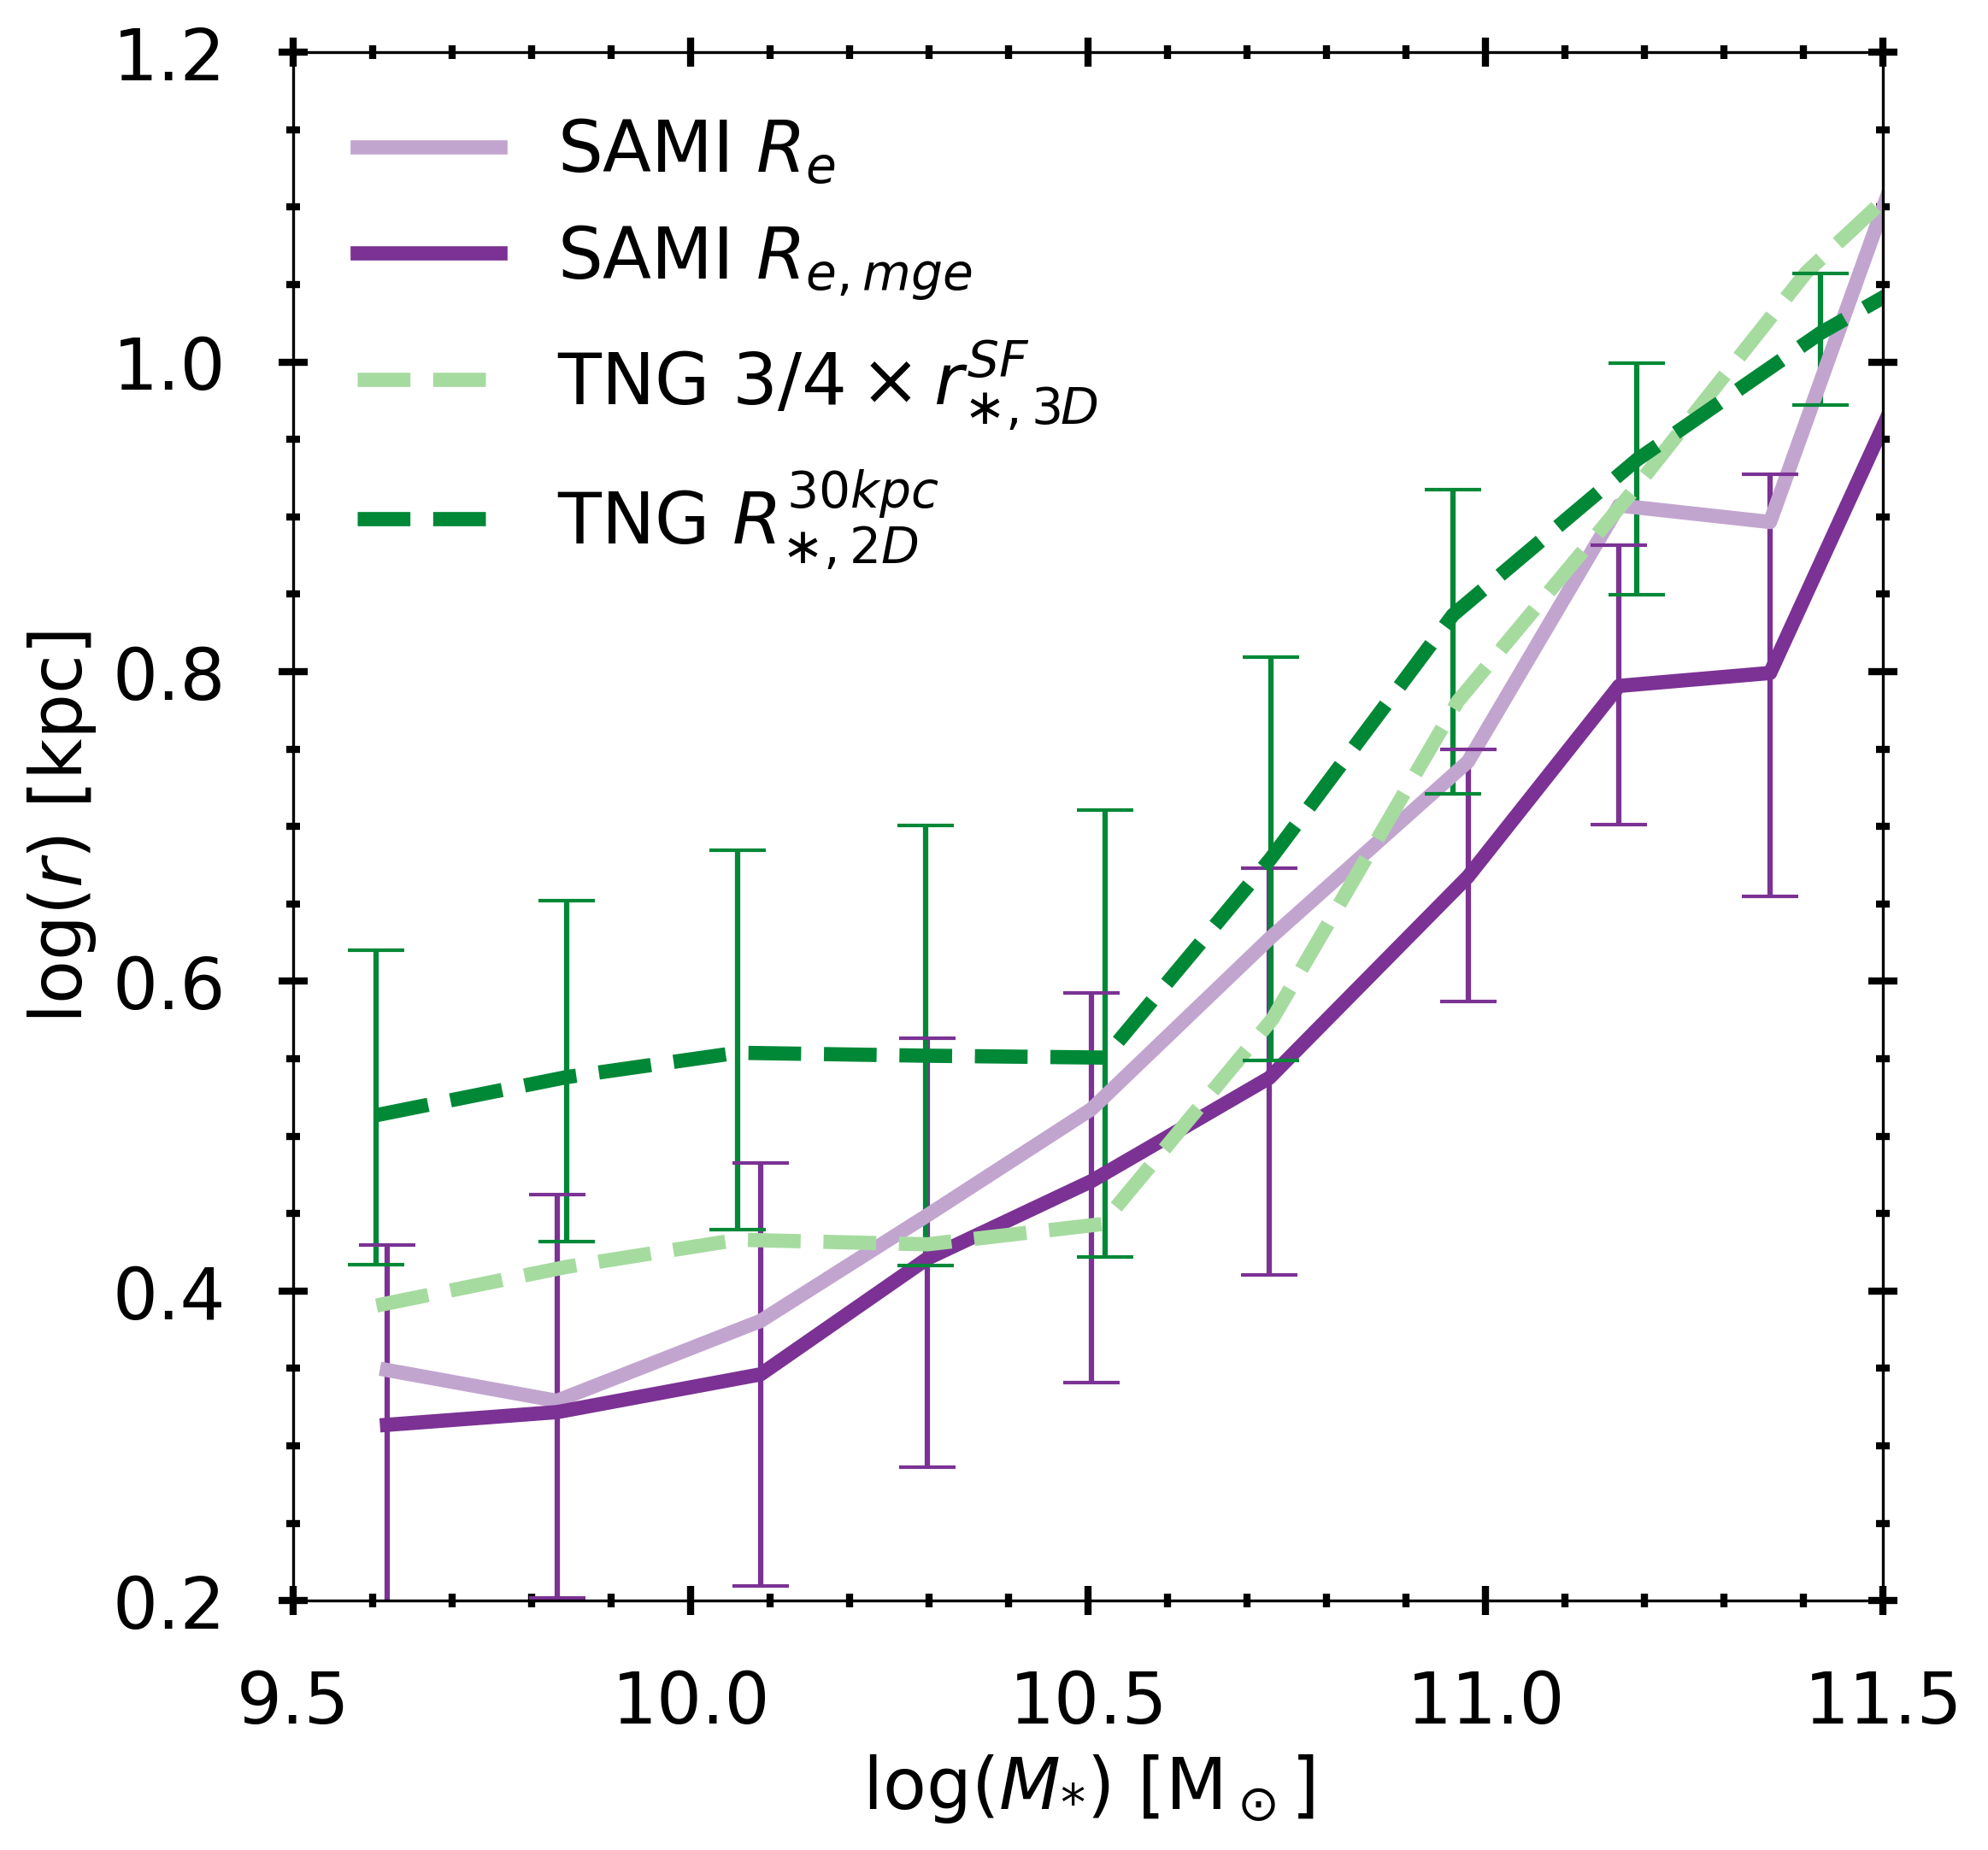
\includegraphics[width=0.9\textwidth]{images/SM_R.png}
    \caption{The size-mass relation of the whole galaxy sample in both TNG and SAMI, given by median values with corresponding 25-75 percentile error bars. TNG values are shown in green dashed lines, while SAMI values are the purple solid lines.}
    \label{SM_R}
\end{figure}

\begin{figure}
    \centering
    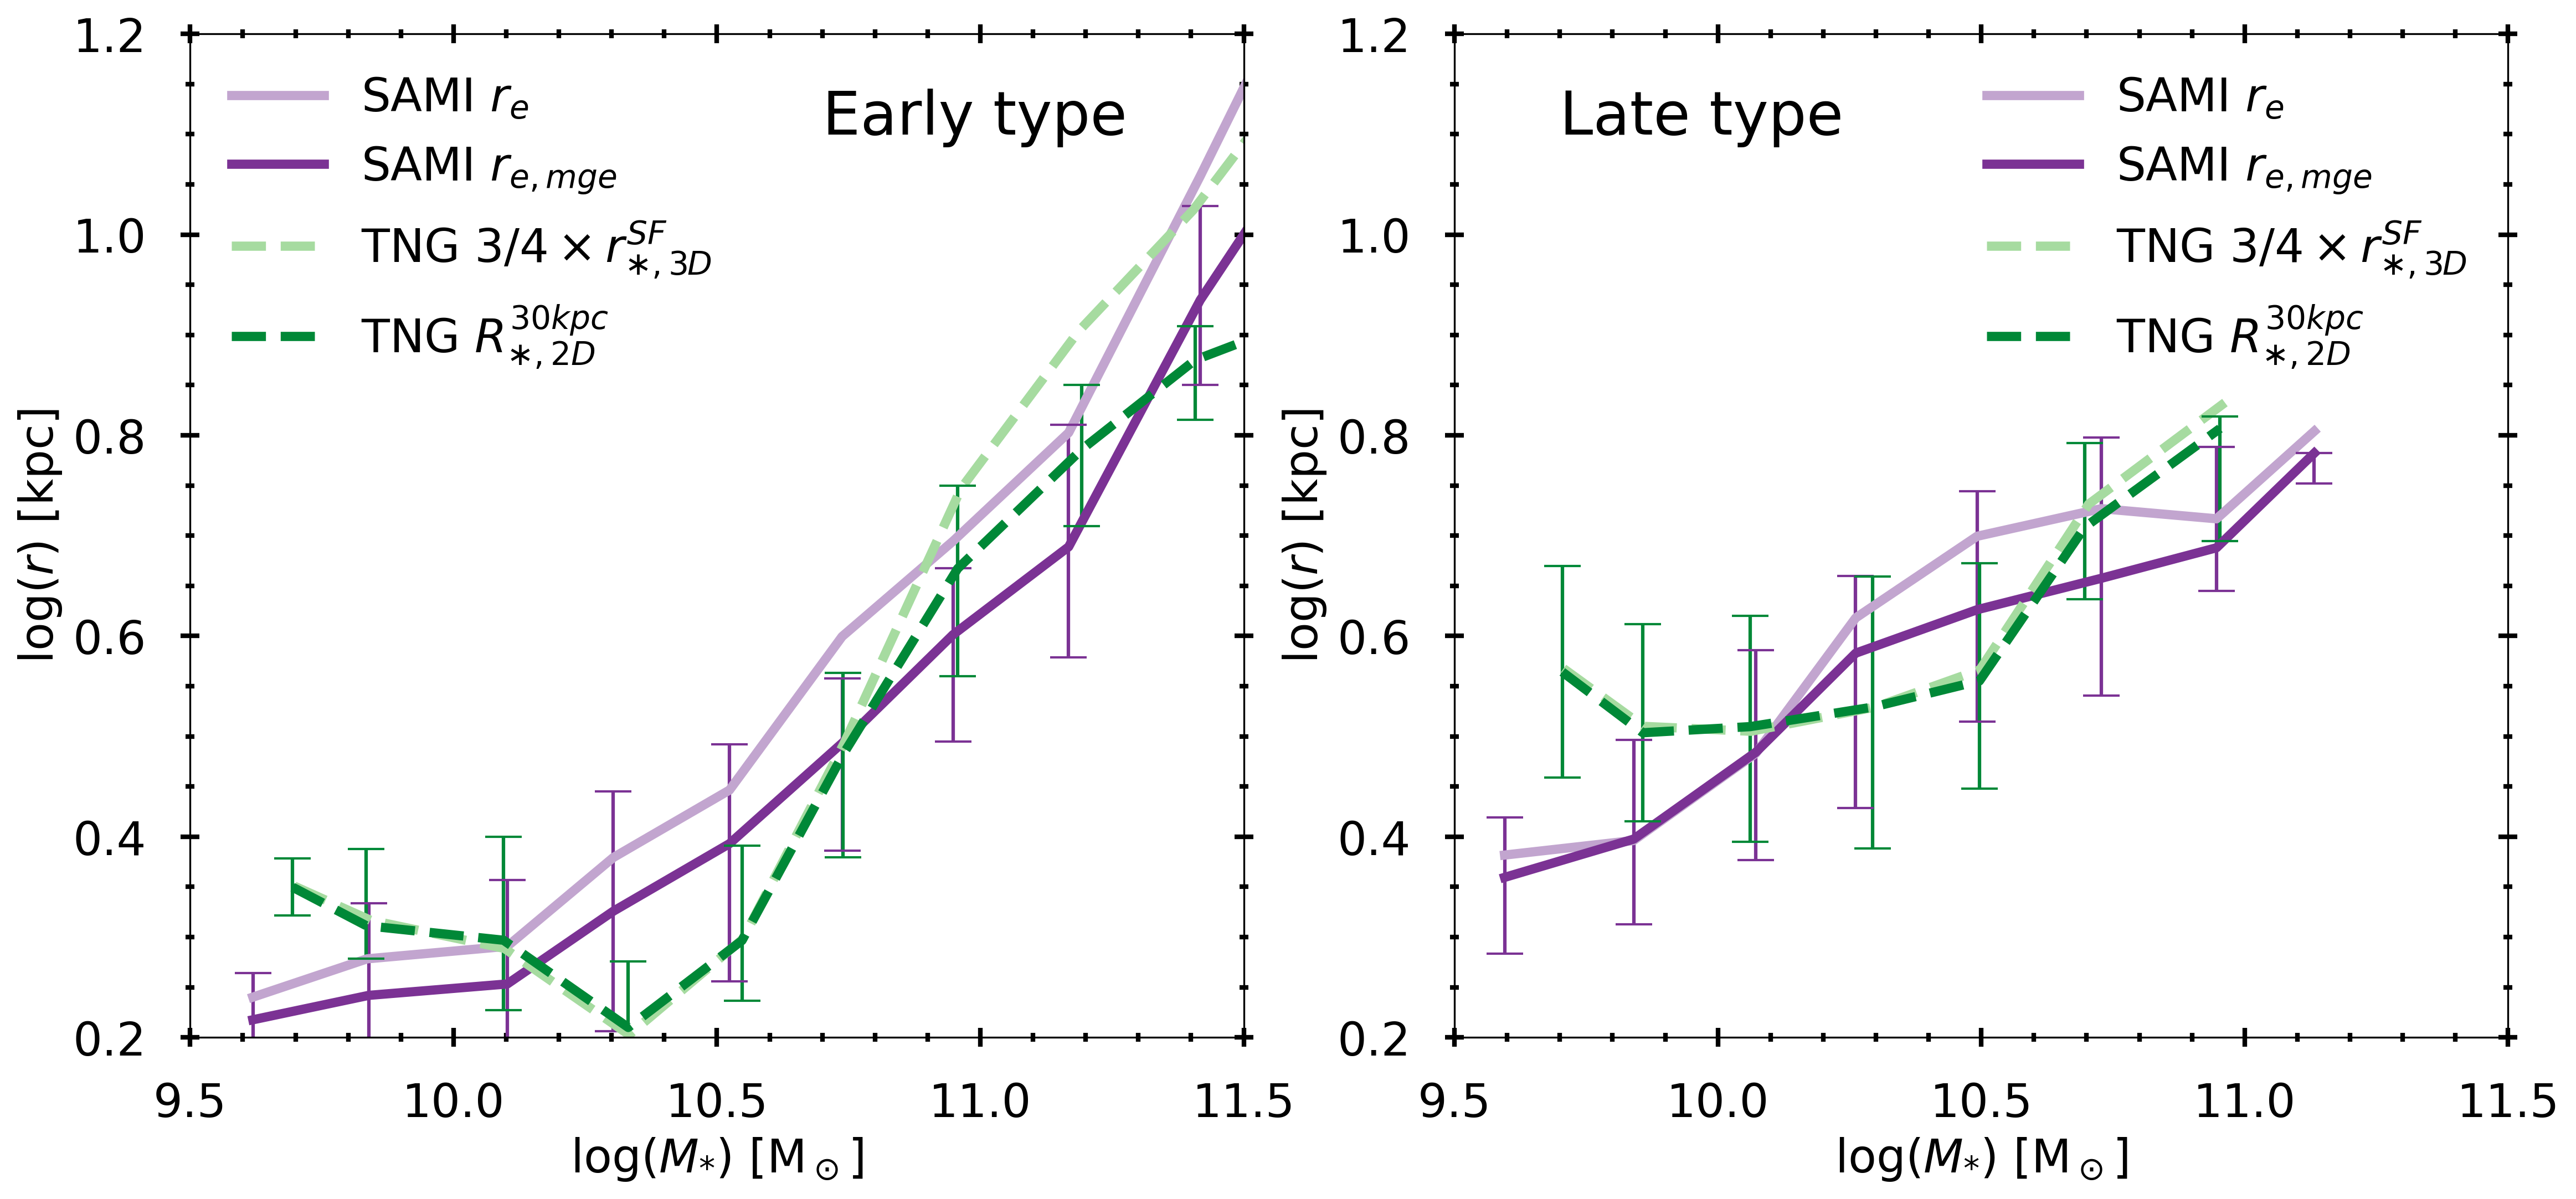
\includegraphics[width=\textwidth]{images/SM_R_morph.png}
    \caption{The size-mass relation of early and late type galaxies in both TNG and SAMI, given by median values with corresponding 25-75 percentile error bars. TNG values are shown in green dashed lines, while SAMI values are the purple solid lines.}
    \label{SM_R_morph}
\end{figure}

\subsubsection{Velocity dispersion}
To investigate the difference between using the particles and the SUBFIND catalog for velocity dispersion estimates, several aspects of how velocity dispersion is calculated must be considered. The SUBFIND value is the mass averaged velocity dispersion of all particles that are bound to the subhalo ($\sigma^{SF}$), while the velocity dispersion measured observationally is either that of stars or that of gas. In Figure \ref{VD_part} the contribution to $\sigma^{SF}$ by the different particles are presented. $\sigma^{SF}$ is the mass averaged sum of these values, and is higher than the baryonic velocity dispersions because of the contribution by the dark matter which dominates the mass contribution in the subhalo. Gas velocity dispersion is lower than $\sigma^{SF}$ by more than 20 \%, and reaching 40 \% in the highest mass galaxies. Thus, using $\sigma^{SF}$ as a proxy for $\sigma_{gas}$ might not be advisable. The stellar velocity dispersion is much closer to $\sigma^{SF}$, being less than 10 \% smaller for all stellar masses. 

Looking further at the stellar velocity dispersion, the effect of a limit on the galaxy size was studied. The results show that there is little to no difference in velocity dispersion values, even at an aperture as small as 10 kpc. Also, the effect of calculating the projected velocity dispersion in three orthogonal directions was compared to scaling the 3D velocity dispersion by a factor of $1/\sqrt{3}$. The difference was neglible for early type galaxies, but the projected quantities were about 10 \% smaller for late types. This is as expected, because early type galaxies are much more spherically symmetric in nature than late type galaxies which are highly anisotropic structures. 

\begin{figure}
    \centering
    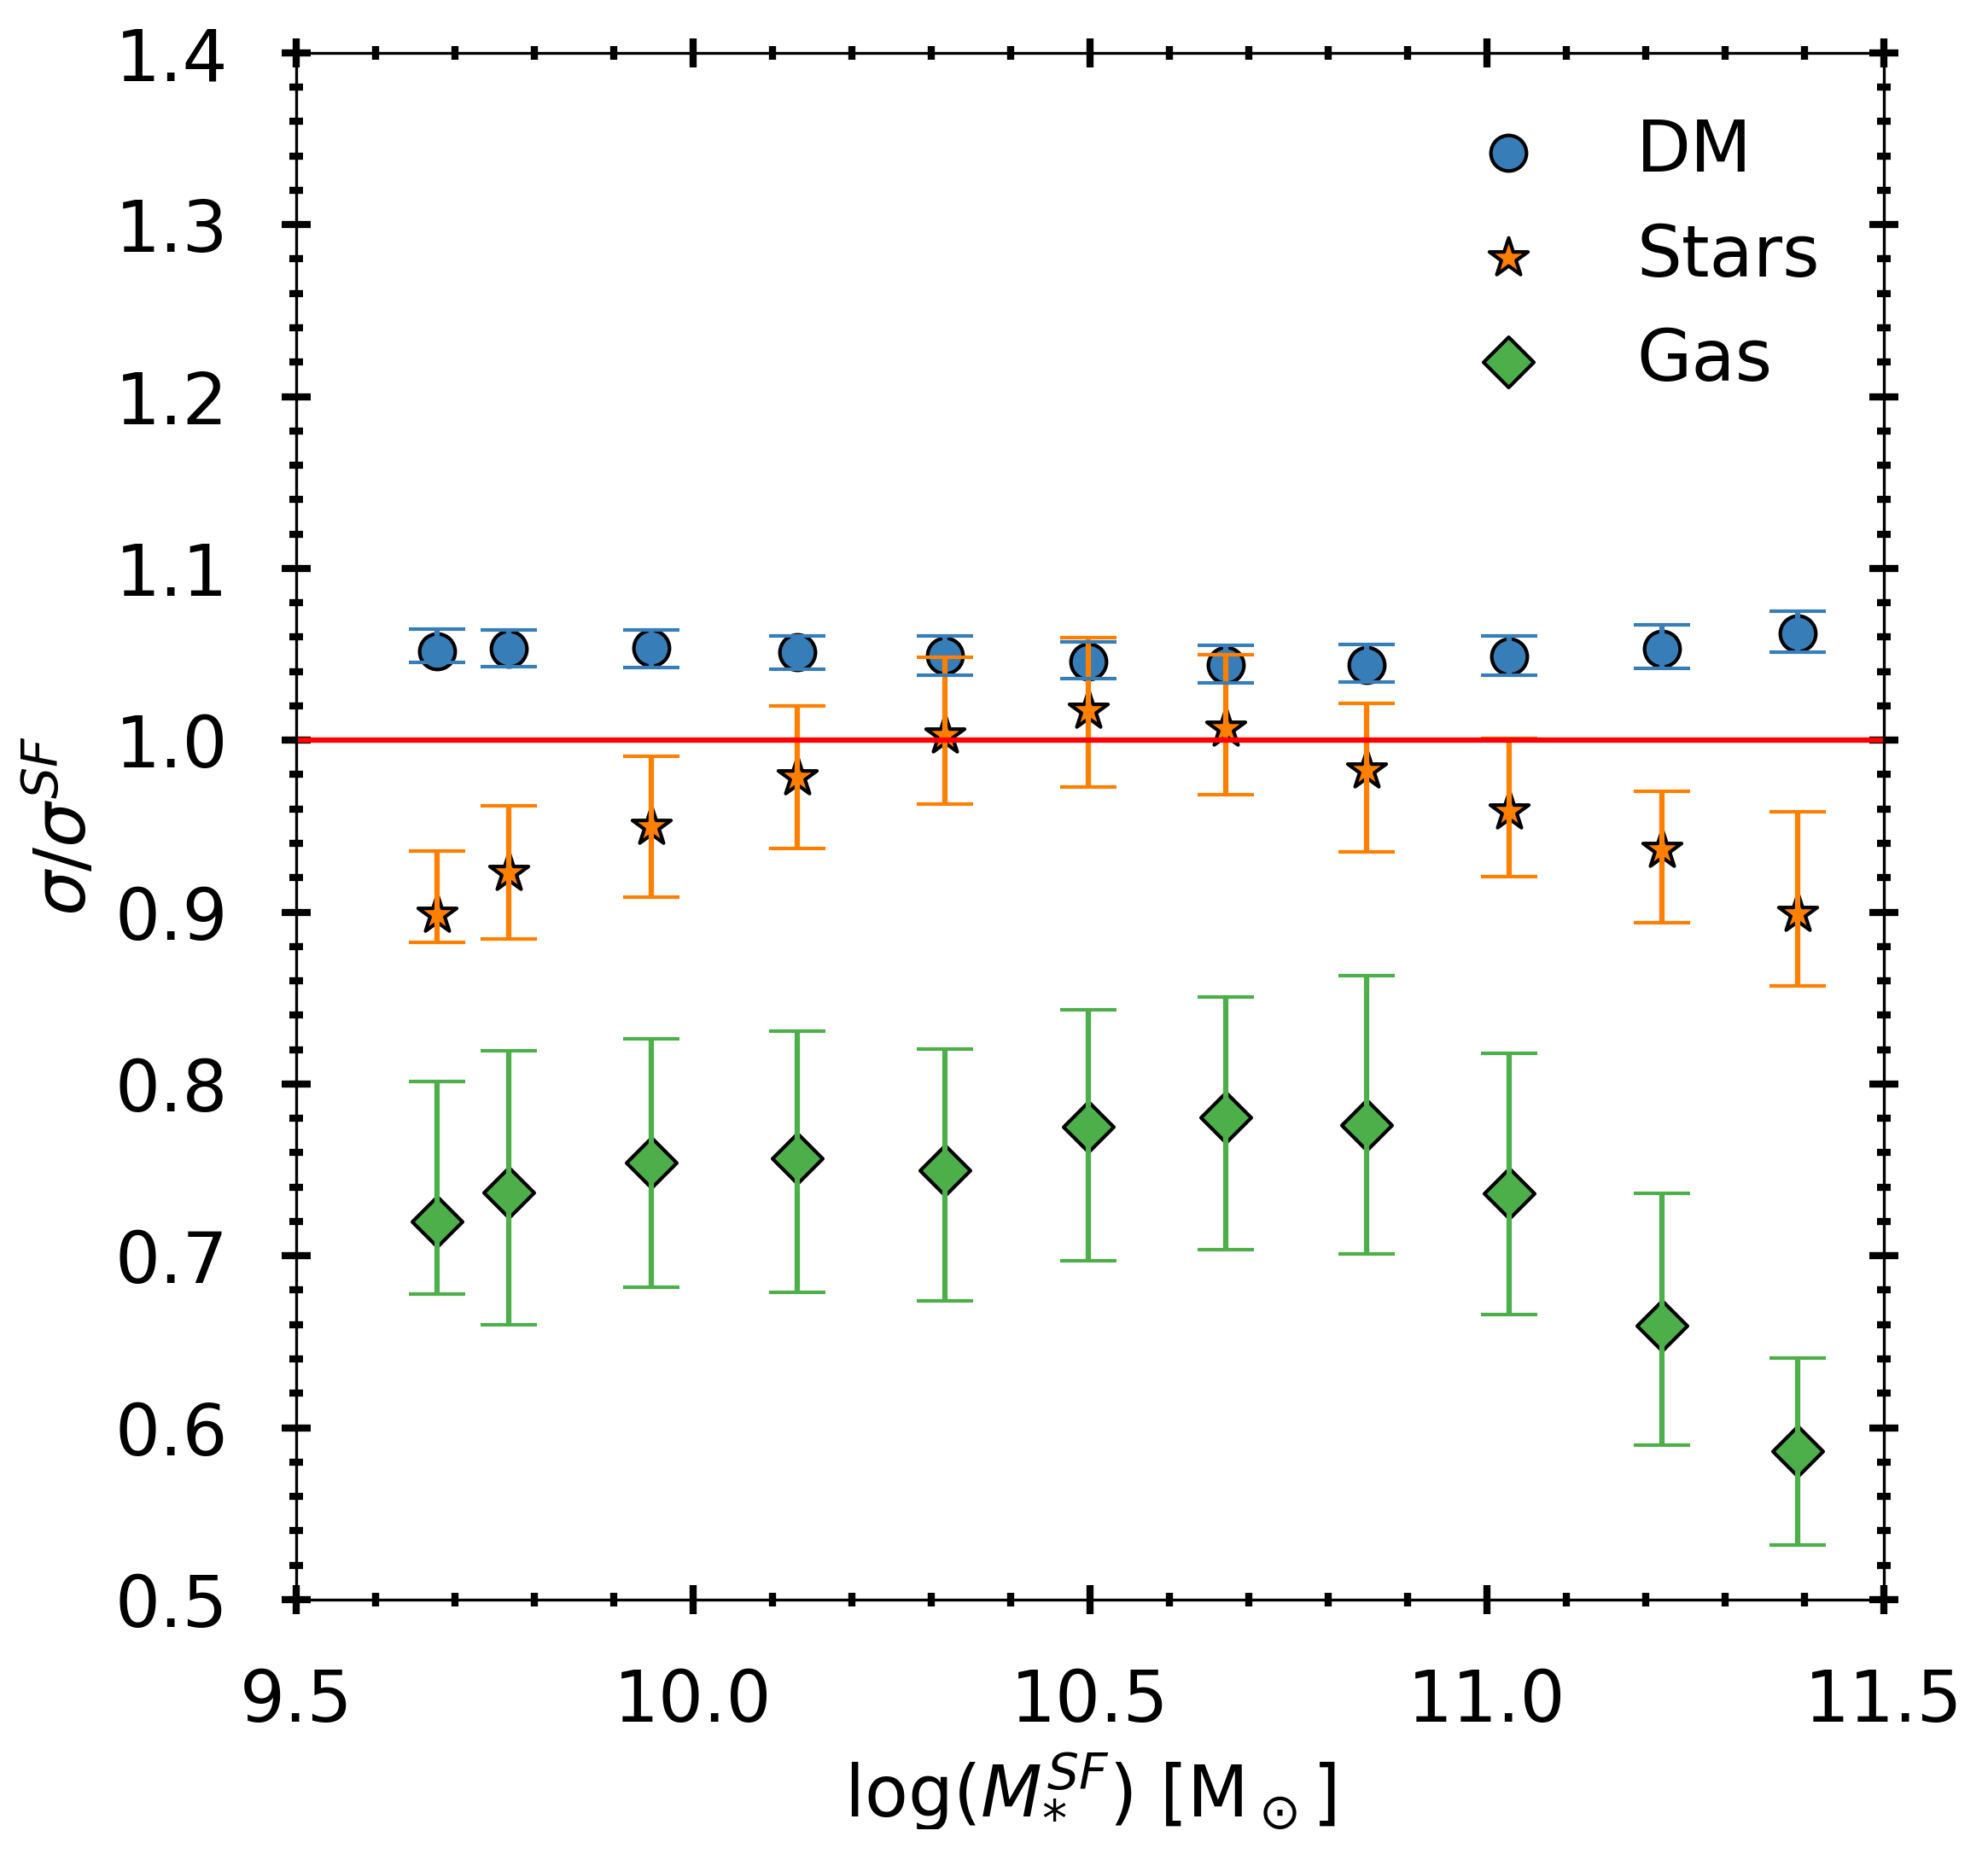
\includegraphics[width=0.9\textwidth]{images/VD_particles.png}
    \caption{Velocity dispersion plotted as function of mass for particles bound to TNG subhalos as identified by SUBFIND. Median values with 25-75 percentile error bars are shown for dark matter (blue circles), stellar particles (orange stars) and gas cells (green diamonds).}
    \label{VD_part}
\end{figure}


The Faber-Jackson relation for early type galaxies is shown in Figure \ref{FJ}. The big difference from SUBFIND results does not come from changing the velocity dispersion definition, but by using a different mass definition. We still get lower velocity dispersion in TNG compared to SAMI, but just by 0.05 - 0.1 dex. It is tempting to contribute the discrepancy to the difference in stellar mass, however by looking at the SHMR relation in Figure \ref{shmr} we see that the mass deviates from observations at around $10^{11} M_{\odot}$, while in Figure \ref{FJ} the difference starts much earlier. Also, the mass is only off from the observations by about 0.1-0.2 dex, but starting at $10^{10.5} M_{\odot}$ the difference from SAMI in the Faber-Jackson relation is larger, up to 0.4 dex at the highest masses. From this, it would seem that velocity dispersions in TNG are lower than those seen in observations at redshift $z=0$. Based on the above analysis, it does not seem like this can be attributed to projection effects or the size of the volume within the velocity dispersion is calculated, but rather the velocities of the simulated stellar particles are in general lower than that which is observed in the stars of real elliptical galaxies.

\begin{figure}
    \centering
    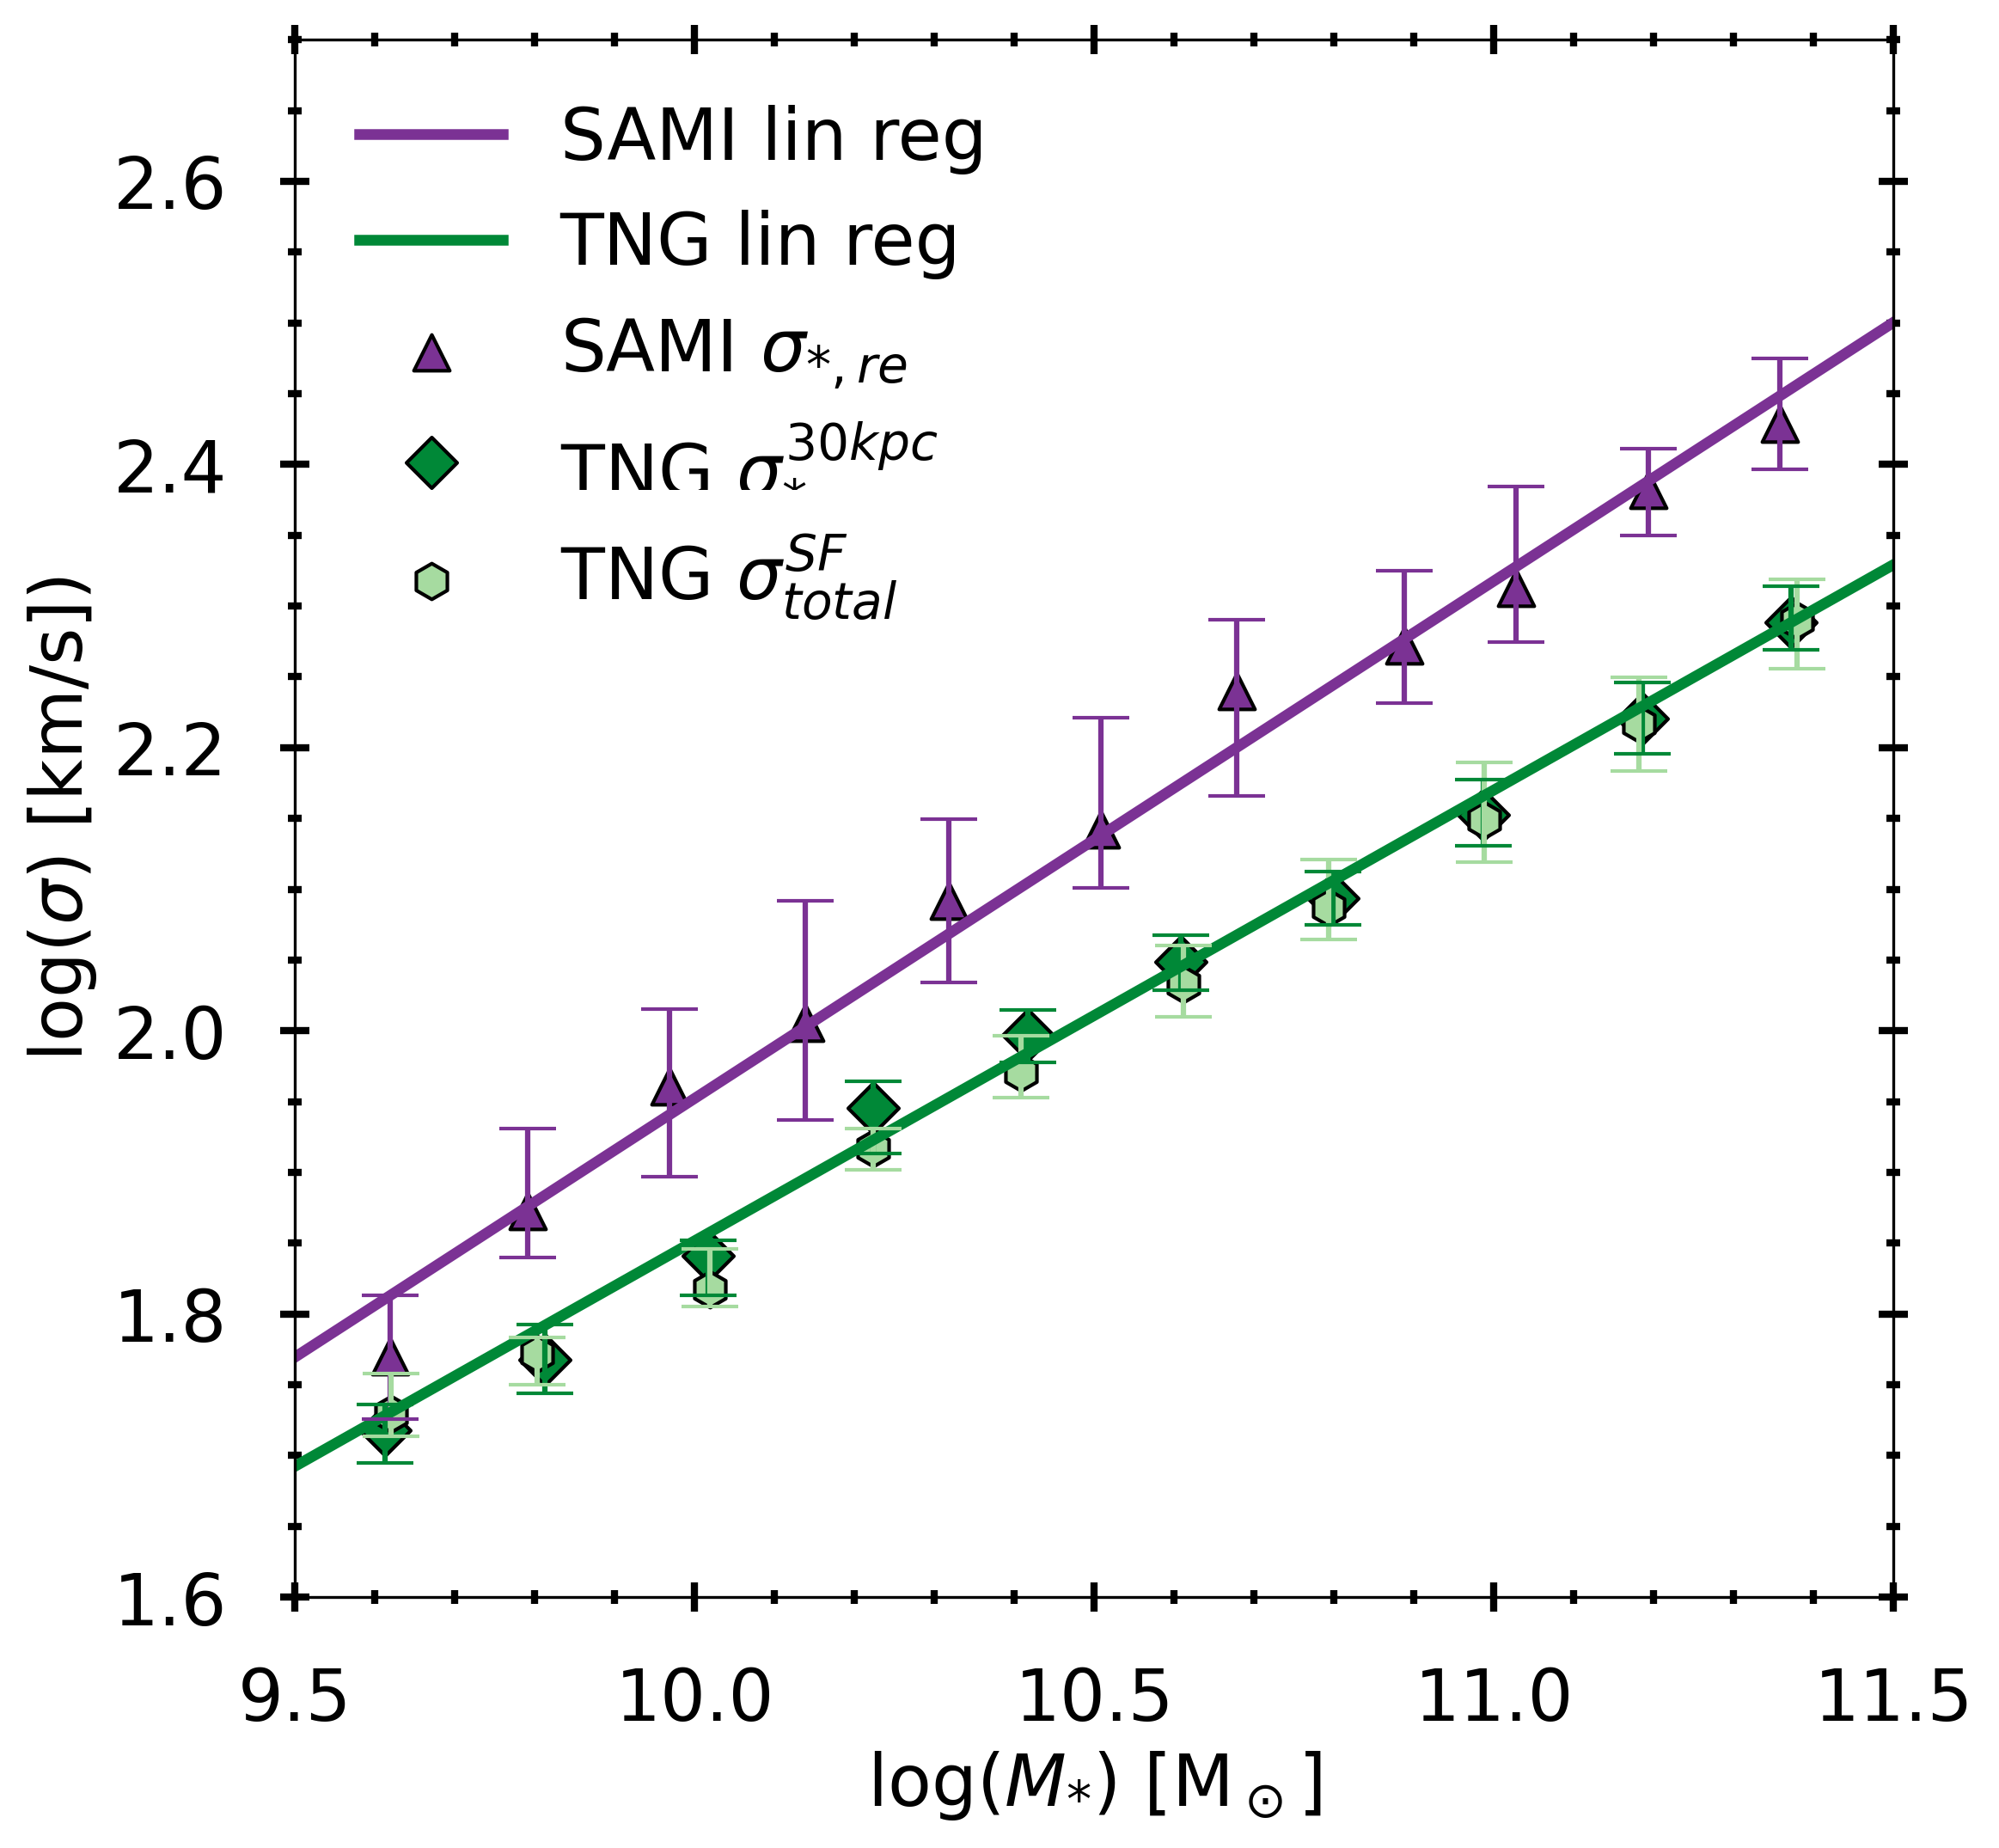
\includegraphics[width=0.9\textwidth]{images/FJ.png}
    \caption{The FJ relation in early type galaxies given by median points with 25-75 percentile error bars for for TNG (dark green points) and SAMI (purple points). Also included are the median points and error bars for the SUBFIND catalog (light green points). The linear fit to TNG (SAMI) are shown as a solid dark green (purple) line. The slope is 0.32 (0.42) with an intercept at -1.33 (-2.25). }
    \label{FJ}
\end{figure}


\subsubsection{Rotational velocity}
As the SUBFIND catalog value for rotational velocity is the maximum of the spherically averaged rotation curve, it was interesting to see if the rotation curve is significantly smaller at specific radii where observational measurements are made. To test this, the rotational velocity was calculated at a distance of $2.2 \times R_{*, 3D}$. There was no difference in the produced data. At that distance the velocity curve is well into the flat regime caused by the dark matter halo, and so this shows that the maximum rotational velocity is not much different from the flat part.

In Figure \ref{TFR} the Tully-Fisher relation is shown for TNG, with the best-fit from the SAMI data by \textcite{Bloom2017}. The SAMI data has a stepper slope than the TNG data, being 0.31 and 0.25 respectively. As late type galaxies generally don't exceed $M_* = 10^{11} M_{\odot}$, we do not expect to see any difference in the TFR for galaxies with apertures 15\% of virial radius or 30 kpc. Using the stellar mass measurement within $2 \times R_{*, 3D}^{SF}$ would decrease the slope further. The SAMI fit is based on a sample of galaxies that span a mass range of $10^{7.5} M_{\odot} - 10^{11.5} M_{\odot}$, but the TFR extends across the stellar range, with a higher scatter at low stellar masses. It would seem then that TNG produces galaxies with lower characteristic rotational velocities than observations show at high mass, and higher velocities at low mass. In other words, the smaller late type galaxies are too compact while the larger are too diffuse. This is something which would be interesting to study in the future.

\begin{figure}
    \centering
    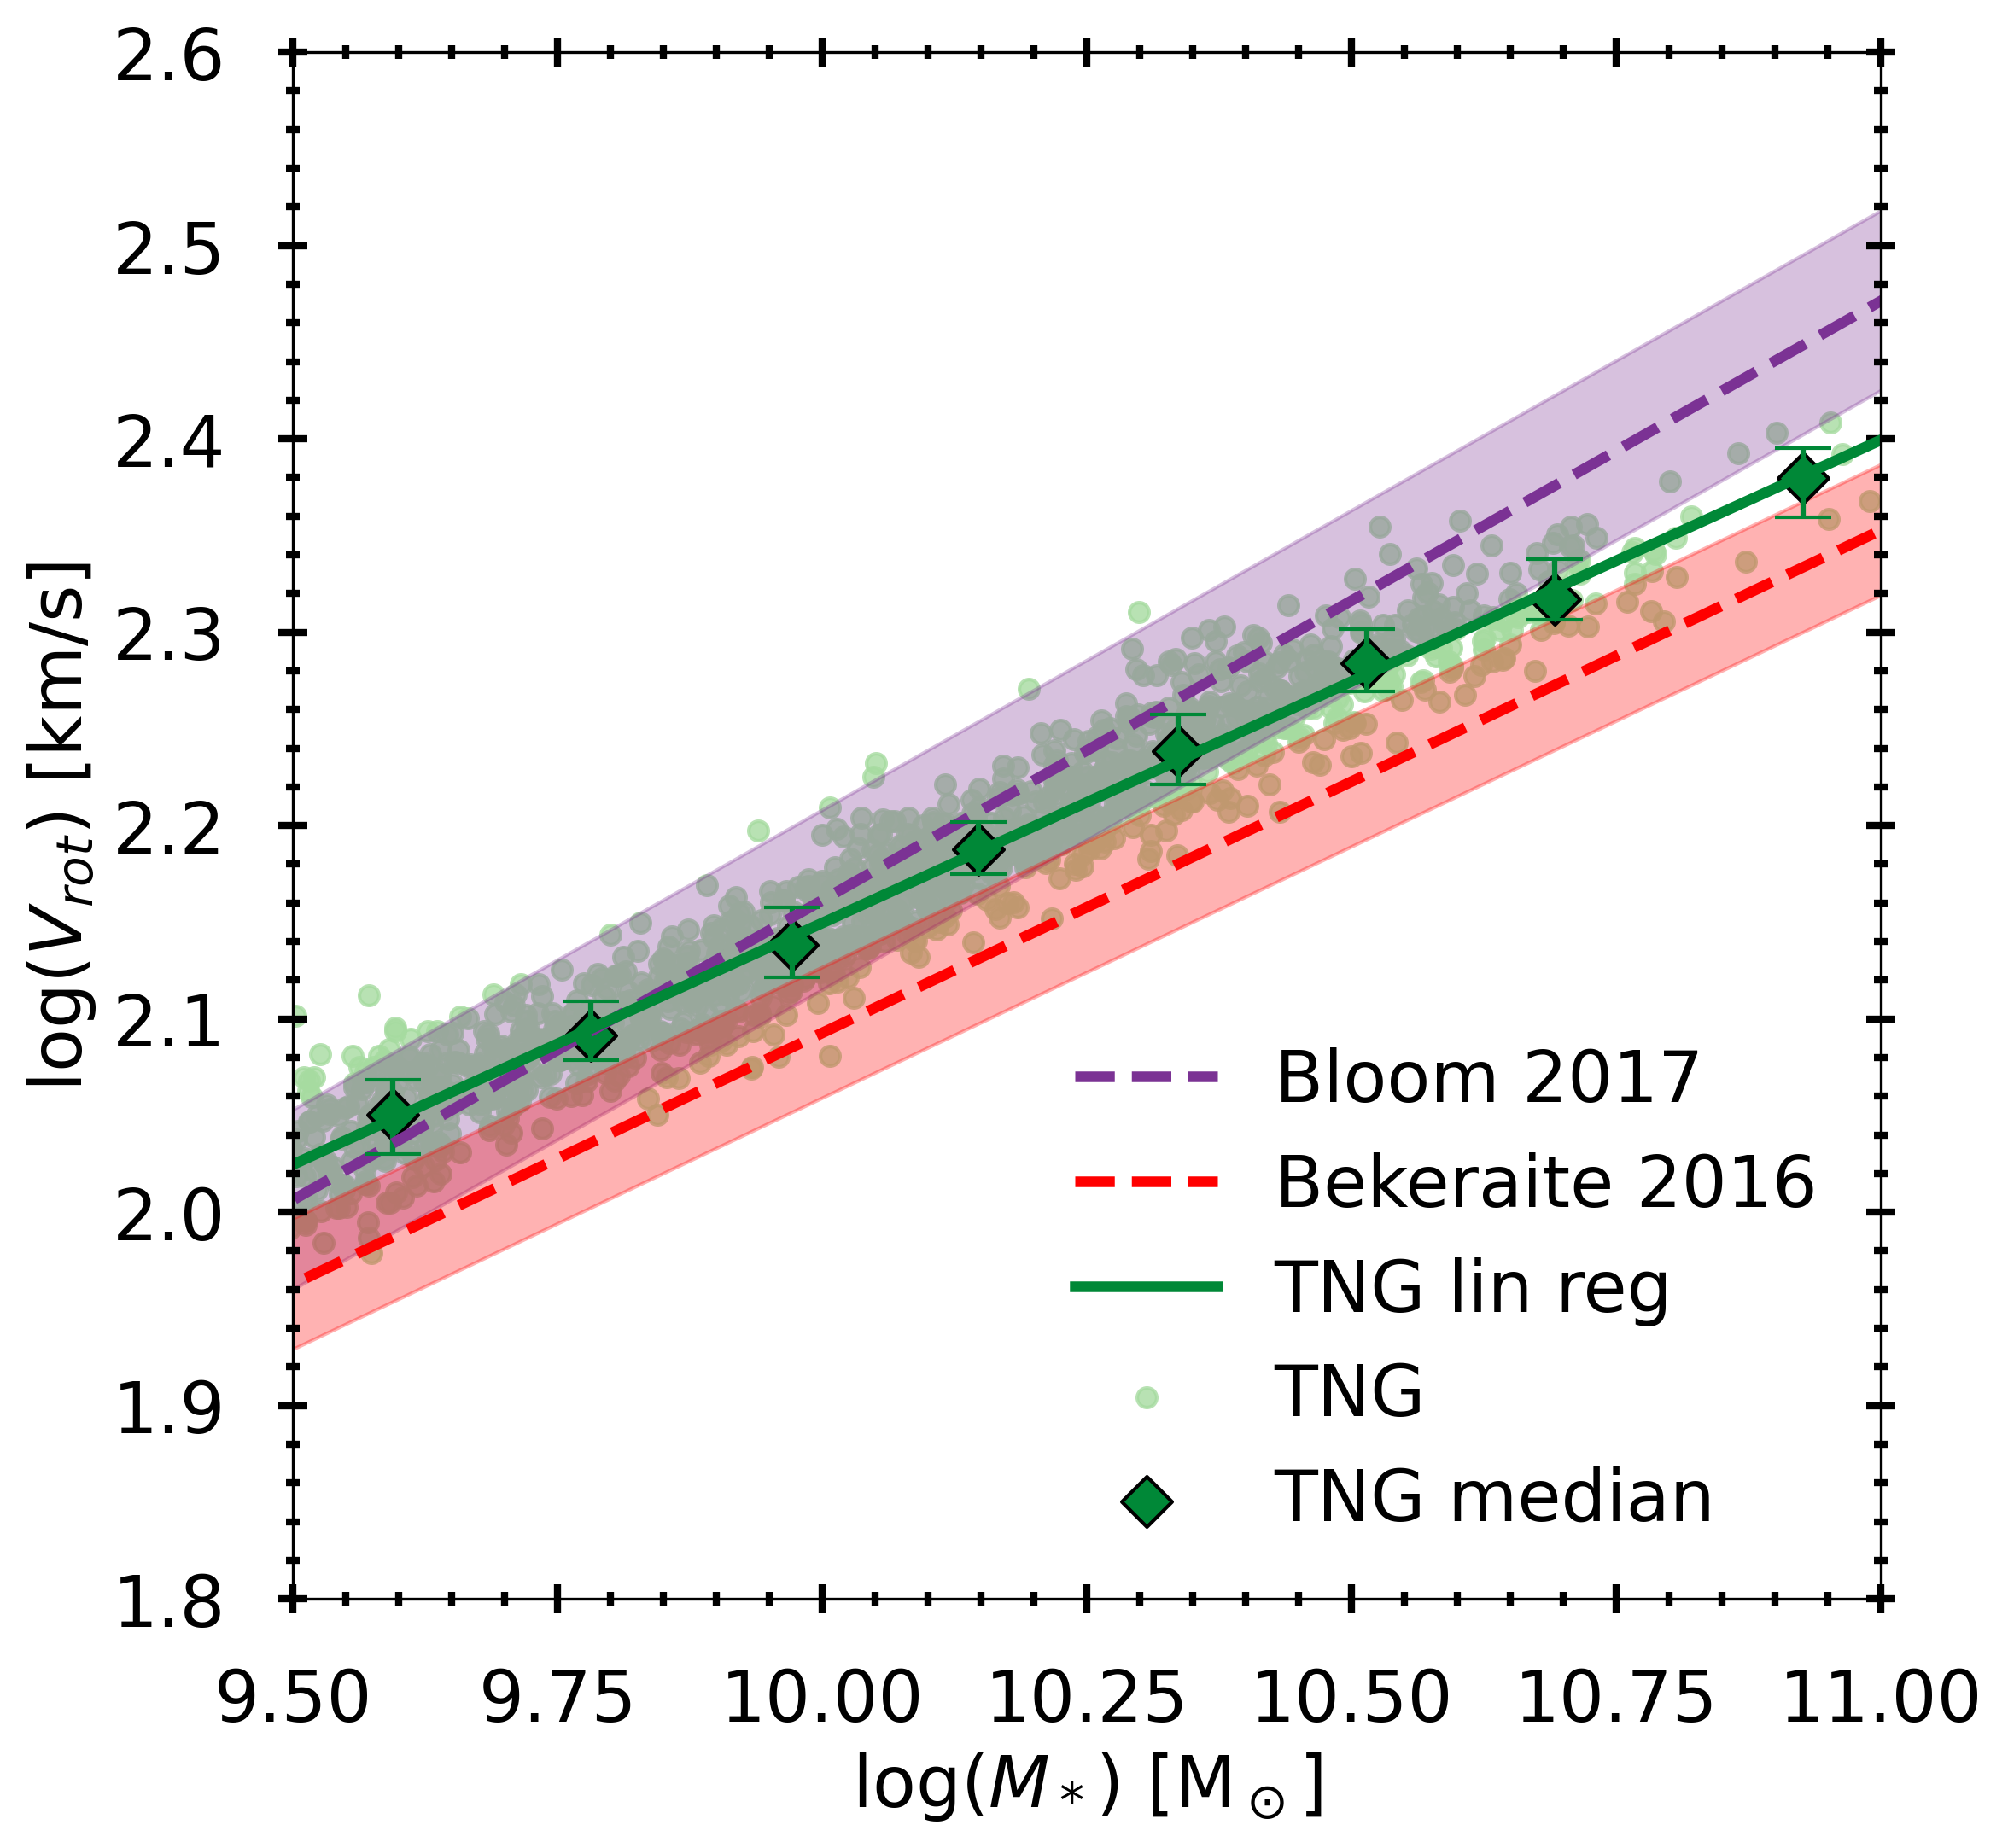
\includegraphics[width=0.9\textwidth]{images/TFR.png}
    \caption{The TFR for TNG (green dots). The median points for TNG are plotted with error bars, showing the 25-75 percentile. The TNG linear fit is also provided (green solid line), it has a slope of 0.25 and an intercept at -0.35. To compare with observations, the best fit for the SAMI data from \textcite{Bloom2017} is shown (purple dashed line). It has a slope of 0.31 with an intercept at -0.94 }
    \label{TFR}
\end{figure}

\subsection{Color bimodality}

Look at PDF for different band widths for whole subhalo (SUBFIND) and for smaller galaxy sizes (particles).
Compare color-mass diagram against SAMI.
Compare PDF against sami for g-i color.

